\section {Технологический раздел}
Для проверки работоспособности схемы необходимо собрать статистически значимое число образцов. 
VirusShare (www.virusshare.com) предоставляет доступ к коллекции вредоносных образцов за 2011-2015, полученных от различных производителей антивирусов, HoneyPot'ов и других источников, собранных в пачки по 65536 штук.
MalShare Project (api.malshare.com/) предоставляет доступ на скачивание  всего до 1000 образцов из их хранилища в день, однако у них новые образцы появляются практически ежедневно.

В связи с этим, было принято решение о первоначальном сборе данных на пачках из VirusShare (<<тренировочная>> выборка) и последующей проверке обнаружения цепочек на собираемых ежедневно с начала 2016 года образцов из MalShare (<<тестовая>> выборка). В связи с имеющимися в наличии ресурсами представляется возможным прогнать всего порядка 60000 штук, поэтому разделим выборки на 56634 vs 7657 штук.

После сбора логов и преобразования становится возможным проследить некоторые тенденции в собранных данных. Если посмотреть на рис. \ref{fig:seq_len_hist}, видно, что значительную часть собранных цепочек составляют те, у которых число вызовов 132 и менее. Скорее всего, большая часть из них относится к тем образцам, у которых по тем или иным причинам не удалось собрать достаточно полную картину вызовов, будь то из-за внезапного завершения работы, проблем обнаружения точки входа упакованных образцов, или каким-либо иным. Длина цепочек большей длины приблизительно соответствует по форме нормальному распределению, а при увеличении числа образцов следовало бы ожидать большей схожести.

\begin {figure}[ht]
        \centering
        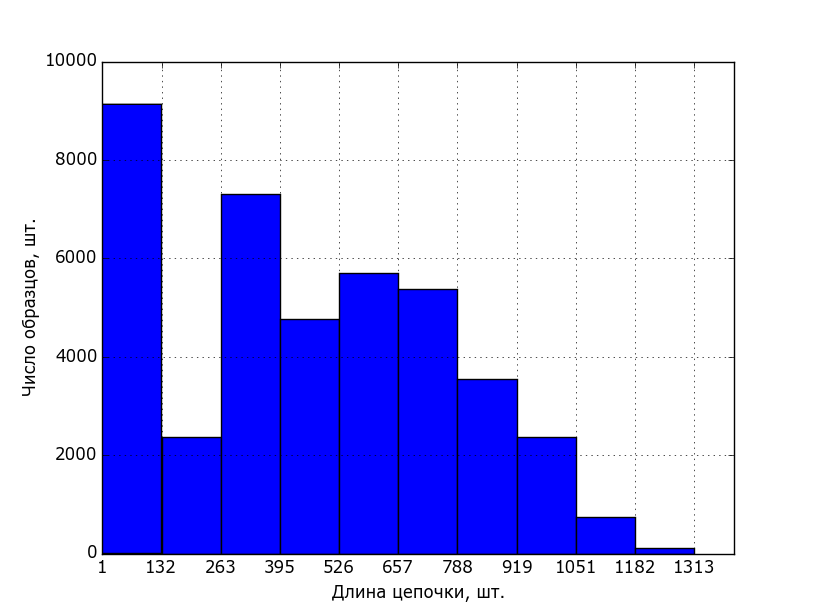
\includegraphics[width=\linewidth] {img/sequence_len_hist.png}
        \caption {Распределение длины цепочек среди образцов}
        \label {fig:seq_len_hist}
\end {figure}

При сравнении цепочек вызовов можно использовать две формы стратегии:
\begin {enumerate}
	\item Быстрая - задание порога, при котором оценка совпадения считается подозрительной. Сравнение с образцами из <<тренировочной>> выборки завершается, как только будет найдено первое подозрительное совпадение, превышающее порог. Это позволяет ускорить сравнение <<тестовой>> выборки. 
	\item Медленная - сравнение с образцами из <<тренировочной>> выборки осуществляется всегда полностью, при этом запоминается максимальные N (например, 3) по оценке совпадения. Это позволяет более точно найти максимально похожие и возможно различные цепочки среди известных, однако сканирование будет занимать максимально возможное время для каждого образца.
\end {enumerate}

Чтобы продемонстрировать возможность обнаружения разных цепочек из одного вируса в других, было выбрано несколько образцов из <<тестовой>> выборки и к ним применена медленная стратегия сравнения.

Первый исследуемый образец имеет хэш f2b6f4793a2f15ee4fafd95d48d78d55. В результате, одним из похожих найденных образцов (самая популярная функция в обнаруженной цепочке --- LoadString) <<тренировочной>> выборки является VirusShare\_0002422da43f24e30470fa08f294acbe, который в классификации Dr. Web'а был определён, как Trojan.DownLoad2.19273, другой (самая популярная функция в цепочке --- ReadFile) - VirusShare\_060f15001381480ff0954366c3315d87, который в  классификации Dr. Web'а определяется, как Trojan.Siggen2.22967. Сам же проверяемый образец по той же самой классификации относится к Program.Unwanted.889.

Хэш другого образца 002f78e9659e185e5bf61c4fd846550a. В результате, один из имеющих с ним сходства образцов в <<тренировочной>> выборке это VirusShare\_00317b3523b195602223ddd038766680, который в классификации Dr.Web'а называется, как Trojan.OutBrowse.1406, другой - VirusShare\_11e949b85a8482b14e8c0329d99e1740, имеющий в той же классификации наименование Adware.Plugin.209.

При использовании быстрой стратегии сравнения общий процент нахождения в <<тестовой>> выборке образцов с оценкой совпадения цепочек более 160 составил 6255/6710 = 93,2 \%. Однако, при этом стоит учитывать отсутствие настройки параметров алгоритма на ложные позитивные срабатывания (единственное, что было сделано в этом смысле - в матрице весов обнулена оценка совпадения вручную выбранных вызовов, имеющих низкую информативность,  например, таких, как InterlockedDecrement - атомарное уменьшение переменной, GetLastError - получает код ошибки результата работы последнего вызова в потоке). Такая настройка потребовала бы примерно такого же объёма программ, что и в <<тестовой>> выборке, причём действия каждой из них должны по каким-либо объективным причинам можно было бы принять за доверенные. Кроме того, по итогам срабатываний были использованы данные всего из 68 образцов (при этом ложные позитивные срабатывания могли перекрыть находящиеся расположенные ближе к концу <<тренировочной>> выборки более близкие образцы.

Как можно наблюдать на столбчатой диаграмме, изображённой на рис. \ref {fig:efficiency}, один из образцов имеет почти в 6 больше порождённых цепочек с совпадениями, чем ближайший к нему. Вполне возможно, он просто обладает некой распространённой последовательностью вызовов, свойственной определённым средам разработки, но сказать точно без проведения дополнительного исследования сложно.
    
\begin {figure}[ht]
	\centering
	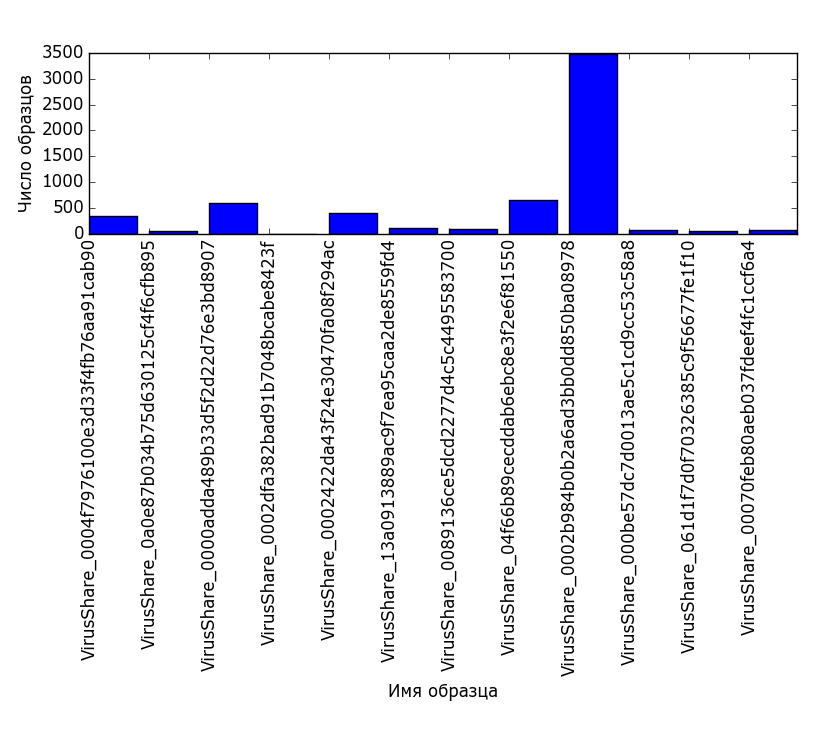
\includegraphics[width=\linewidth] {img/most_used_kbase_samples.png}
	\caption {Участвовавшие в совпадениях образцы из <<тренировочной>> выборки}
	\label {fig:efficiency}
\end {figure}

В итоге, мы всё равно получаем возможность утверждать, что предложенный подход и реализация имеют возможность практического применения, а также возможна настройка полноты и точности алгоритма при использовании признанных не несущими вредоносную нагрузку тренировочных образцов с целью уменьшения срабатывания на распространённые в ПО общего назначения цепочки вызовов.